\section{Jarosław Mastalerczyk}

\section*{Wind contidtions}




\begin{flushleft}
\underline{The faster} the average \textbf{wind speed}, the more electricity the wind turbine will generate, so faster winds are generally economically better for wind farm developments. \par
The balancing factor is that strong gusts and high turbulence require stronger more expensive turbines, otherwise there is a \textbf{risk of damage}. The average power in the wind is not proportional to the average wind speed. For this reason, the ideal wind conditions would be strong but consistent winds with low turbulence coming from a single direction. \par
\end{flushleft}


World's 3 largest onshore wind farms:
\begin{itemize}
  \item Gansu wind farm
  \item Zhang Jiakou
  \item Urat Zhongqi, Bayannur City
\end{itemize}


World's 3 largest onshore wind farms:
\begin{enumerate}
  \item Gansu wind farm
  \item Zhang Jiakou
  \item Urat Zhongqi, Bayannur City
\end{enumerate}

\begin{figure}[htbp]
    \centering
    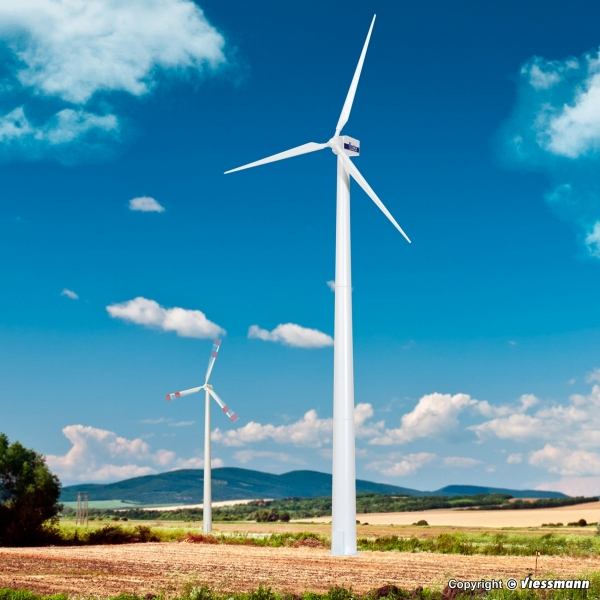
\includegraphics[width=0.4\textwidth]{pictures/wiatrak.jpg} 
    \caption{Wiatraki sa eko.}
    \label{fig: wiatrak}
\end{figure}



Table~\ref{tab:weekend} represents ile godzin spalem w weekend.






\begin{table}[ht]
\centering
\begin{tabular}{|l|l|}
\hline
\textbf{TABELA ILE GODZIN SPALEM W  WEEKEND} &   \\ \hline
PT                                           & 6 \\ \hline
SB                                           & 5 \\ \hline
ND                                           & 4 \\ \hline
\end{tabular}
\caption{W tabeli widać, że snu bylo za malo.}
\end{table}

\label{tab:weekend}
Calka : \[ \int{a}^{b} x^2 \,dx \]